\newpage
\section{USART (Universal Synchronous-Asyncronous Receiver-Transmitter)}

L'USART (Universal Synchronous-Asyncronous Receiver-Transmitter) è un interfaccia di comunicazione seriale. In generale i sistemi di comunicazione seriale utilizzano solo 1 filo per comunicare (Tx -> Rx), che permette il collegamento tra il trasmittente ed il ricevente, a questo singolo collegamento, solitamente, si aggiungono altri fili, che aggiungono: controlli di flusso, segnali di tempificazione ecc.
Non si scende troppo nei dettagli di tali architetture, poichè poi si vanno a specializzare nei vari dispositivi che vengono prodotti, un esempio sarà l'Intel 8251.

\subsection{Comunicazioni Sincrona ed Asincrona}
Come detto nel precedente paragrafo, l'USART (a differenza del suo predecessore, l'UART), prevede 2 modalità di funzionamento:
\begin{itemize}
    \item \textbf{Sincrona}
    \item \textbf{Asincrona}
\end{itemize}
Tali modalità sono profondamente diverse, sia per quanto riguarda l'architettura sia per quanto riguarda il loro modo di comunicazione dei dati.

\subsubsection{Comunicazione Sincrona}
Nel caso della comunicazione di tipo Sincrona, i due dispositivi (per una comunicazione unidirezionale) condividono 2 collegamenti:
\begin{itemize}
    \item Tx -> Rx
    \item clk\_t -> clk\_r
\end{itemize}

Questo perchè una comunicazione sincrona sfrutta un segnale di tempificazione comune. La velocità di trasmissione dei dati è quindi dettata dalla frequenza del clock comune. A differenza della comunicazione \textbf{asincrona}, la comunicazione sincrona è molto più veloce e robusta (data la sincronizzazione in hardware tramite il clock condiviso), ma è molto difficile da implementare a livello hardware, poichè bisogna sincronizzare in maniera molto precisa dati e trasmissione di essi.

\subsubsection{Comunicazione Asincrona}
Nel caso della comunicazione di tipo Asincrona, i due dispositivi richiedono un singolo collegamento (sempre ragionando sul singolo canale trasmissivo Tx -> Rx).
L'invio dei dati è gestito da due bit di start e stop che vanno a scandire, precisamente, l'inizio dell'invio del messaggio e la fine del messaggio.
La tipologia di comunicazione, rispetto alla \textbf{Sincrona} risulta meno efficiente rispetto al trasporto di informazioni, anche se conserva il vantaggio per il rispetto dell'asincronicità intrinseca dei dati, e quindi ottimizza meglio i tempi di invio dei dati (non deve aspettare un fronte del clock condiviso come nel caso della comunicazione sincrona).
Nel caso \textbf{Asincrono}, negli anni 60, è stato definito uno standard di comunicazione, ovvero l'\textbf{RS-232}, uno standard che definisce in che modo le varie interfacce possono comunicare tra di loro, tale standard predispone varie altri tipologie di collegamenti che sono utilizzate per il controllo di flusso dei vari dati. Tale standard fu creato per permettere la comunicazione tra un dispositivo DCE (Data Communication Equipment) ed un dispositivo DTE (Data Trasmission Equipment), tali dispositivi potevano essere tutto, originariamente erano un calcolatore ed il suo modem. Precisamente, i pin che sono presentati ed utilizzati nello standard sono:

\begin{itemize}
    \item \textbf{RD}: Sarabbe il pin di ricezione di dati seriali
    \item \textbf{TD}: Sarebbe il pin di trasmissione di dati seriali
    \item \textbf{DCD}: Data Carrier Detect, è un pin che viene utilizzato per controllare il corretto collegamento tra i due dispositivi (controllo del funzionamento corretto del dispositivo e delle portanti utilizzate)
    \item \textbf{GND}: Ground, è un pin che collega la massa dei sue dispositivi in modo da poter trasmettere il segnale senza intoppi di tipo elettrico
    \item \textbf{DTR}: Data Terminal Ready, indica il segnale di uscita per poter finire/iniziare una fase di handshacking (ACK o SYN)
    \item \textbf{DSR}: Data Set Ready, indica il segnale di ingresso che viene inviato dal ricevente (o per indicare un ACK o un SYN)
    \item \textbf{RTS}: Request to send, segnale di uscita per il controllo del flusso
    \item \textbf{CTS}: Clear To Send, sengale di ingresso per il controllo di flusso
    \item \textbf{RI}: Ring Indicator, Indica che il trasmittente sta "chiamando", solitamente tale pin va a scatenare una interruzione per poter far gestire la comunicazione
\end{itemize}
I segnali \textbf{DTR} e \textbf{DSR}, sono pin che vanno ad implementare l'handshacking ad un livello molto alto. Mentre \textbf{RTS} e \textbf{CTS}, vengono utilizzati per comprendere quando il trasmittente può effettivamente trasmettere. Per quando sia un pò confusionario il loro funzionamento, immaginando una comunicazione dove dev'essere effettuato l'invio di messaggi, il primo handshacking serve ad identificare il messaggio, mentre il secondo per trasmettere i vari byte e quindi richiedere al ricevitore se è pronto a ricevere o sta ancora processando il dato precedente.

\subsubsection{Errori principali presenti nella comiunicazione seriale}
Quando si fanno interagire due sistemi mediante una comunicazione di tipo seriale asincrona (UART), in fase di ricezione, si può andare in contro ai seguenti tipi di errori:
\begin{itemize}
    \item \textbf{Errore di parità}: Il valore del bit di parità inviato non corrisponde con quello calcolato al ricevitore;
    \item \textbf{Errore di framing}: Non è previsto il bit di stop;
    \item \textbf{Errore di Overruning}: Errore dovuto alla differenza dei clock di invio. Se il sistema ricevente è più lento del sistema trasmittente, allora si può avere perdita di informazioni (non si coglie bene il bit di start);
\end{itemize}

Tra questi errori l'unico su cui si può attuare un miglioramento è quello di overrun, questo perchè si può prevedere che il dato venga trasmesso secondo uno specifico protocollo di handshacking. Difatti nelle architetture sono presenti appositi collegamenti per l'implementazione di tale soluzione, anche se quest'ultima rallenta un po la ricezione rendendola meno efficiente.

\subsection{Intel 8251A}\label{par:intel-8251A}
L'Intel 8251A è un dispositivo programmabile che permette la comunicazione tra la CPU e una qualunque periferica seriale che utilizza lo standard RS-232. Tale dispositivo riceve i dati da trasmettere in maniera parallela dalla CPU, per poi inviarli in maniera seriale attraverso l'utilizzo del protocollo selezionato in una prima fase di configurazione (per questo programmabile). 
La sua struttura principale è quella visualizzabile nella figura [\ref{img:Intel-8251A}]

\begin{figure}
    \centering
    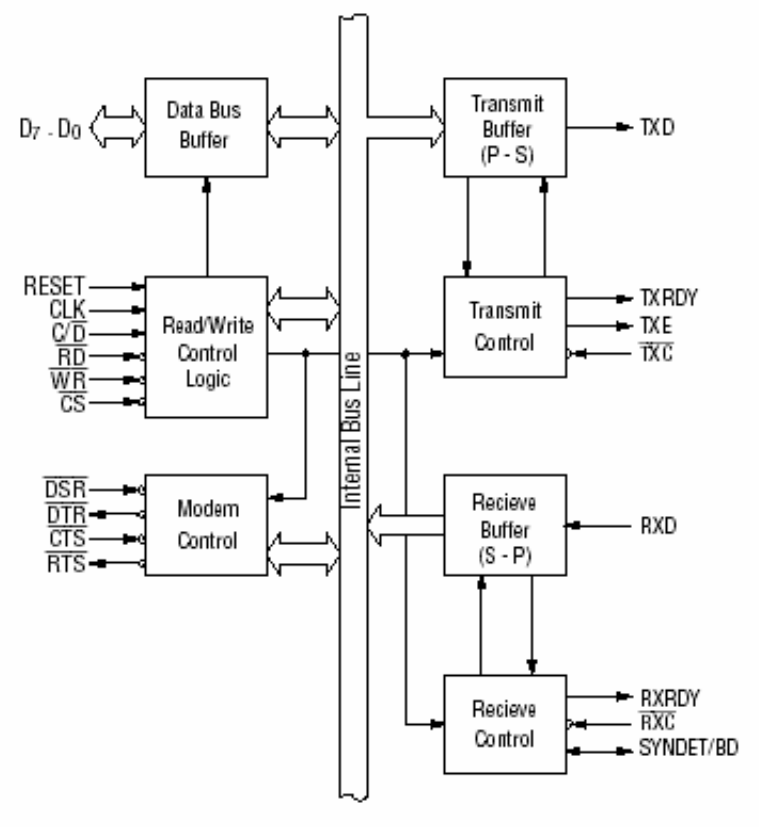
\includegraphics[width=.5\textwidth]{img/Intel8251A.png}
    \caption{Struttura dell'Intel 8251A}\label{img:Intel-8251A}
\end{figure}

In tale struttura logica notiamo vari blocchi differenti, ovvero:
\begin{itemize}
    \item \textbf{Data Bus Buffer}: Buffer in cui vengono conservari i dati (o in ricezione o in trasmissione), in generale la comunicazione con tale blocco avviene in maniera parallela;
    \item \textbf{Read/Write Control Logic}: Componente di controllo dell'intero sistema, va a creare un interfaccia di utilizzo degli elementi interni del dispositivo per la CPU. Vedendo meglio il significato dei vari pin:
    \begin{itemize}
        \item \textbf{Reset}: Pin che permette alla CPU di resettare tutti i registri interni al dispositivo;
        \item \textbf{Clk}: Segnale di tempificazione per il dispositivo;
        \item \textbf{C/D}: Selezione per il registro di controllo o di dato
        \item \textbf{RD e WR}: Segnali che indentificano se si vuole effettuare una lettura o una scrittura
        \item \textbf{CS}: Chip select, utilizzato per abilitare il dispositivo
    \end{itemize} 

    \item \textbf{Modem Control}: Blocco di collegamento con l'altro dispositivo esterno, difatti contiene i segnali che vengono utilizzati per lo standard RS232
    \begin{itemize}
        \item \textbf{DSR (Data Set Ready)}
        \item \textbf{DTR (Data Terminal Ready)}
        \item \textbf{CTS (Clear To Send)}
        \item \textbf{RTS (Ready To Send)}
    \end{itemize}

    \item \textbf{Transmit Buffer}: Contiene lo shift register impiegato nella fase di trasmissione. Gli vengono passati i dati da trasmettere in parallelo dal BUS dati e poi li invia sotto forma seriale tramite il segnale \textbf{TXD}. IL controllo sulla trasmissione viene effettuato dall'apposito blocco con cui si condividono sia un segnale di ingresso che di uscita
    
    \item \textbf{Transmit Control}: Il blocco di trasmit control viene gestito da vari segnali processati, in base alle richieste della CPU. I suoi segnali di interazione con l'esterno, sono:
    \begin{itemize}
        \item \textbf{TXRDY (Transmitter ReaDY)}: Segnale di utilizzato per segnalare alla CPU che il trasmettitore è pronto a ricevere un nuovo dato
        \item \textbf{TXE (Transmitter Empty)}: Segnale di uscita per identificare che il buffer di trasmissione può essere sovrascritto (Attesa del nuovo dato)
        \item \textbf{TXC (Transmitter Clock)}: Utilizzato nel caso sincrono per gestire il segnale di clock condiviso
    \end{itemize}
    
    \item \textbf{Receive Buffer}: Il blocco di receive buffer, svolge il compito contrario del trasmit buffer, ovvero, converte i dati seriali in registro parallelo e li invia sul bus dati. Esso riceve i dati tramite il segnale esterno RXD. Oltre a tale segnale ne ha altri che ne fanno il controllo e la gestione della comunicazione
    
    \item \textbf{Receive Control}: Il blocco di receive control, come il blocco di transmit control, gestite il sistema di ricezione con l'esterno. Tale gestione viene effettuata secondo i seguenti segnali:
    \begin{itemize}
        \item \textbf{RXRDY (Receive Ready)}: Specifica alla CPU che il sistema ricevente ha ricevuto un dato che è pronto per essere letto
        \item \textbf{RXC (Receive Clock)}: Segnale utilizzato in ingresso per il clock delle comunicazioni sincrone
        \item \textbf{SYNDER/BD (Synchronous Detect/Break Detect)}: Segnale utilizzato per, nel caso di comunicazioni sincrone, ricevere i caratteri di sincronismo, mentre nella modalità sincrona segnala la rilevazione di una congizione di breack
    \end{itemize}
\end{itemize}

\subsubsection{Intel-8251A in Asim}
Come detto in precedenza, l'Intel 8251A è un dispositivo programmabile, quindi richiede di una prima fase di configurazione (tramite il suo registro di modo) e poi il suo utilizzo tramite gli altri registri dell'interfaccia. Nel caso di ASIM il modello di programmazione utilizzato è quello visualizzabile alla figura [\ref{img:prog-8251A}]

\begin{figure}
    \centering
    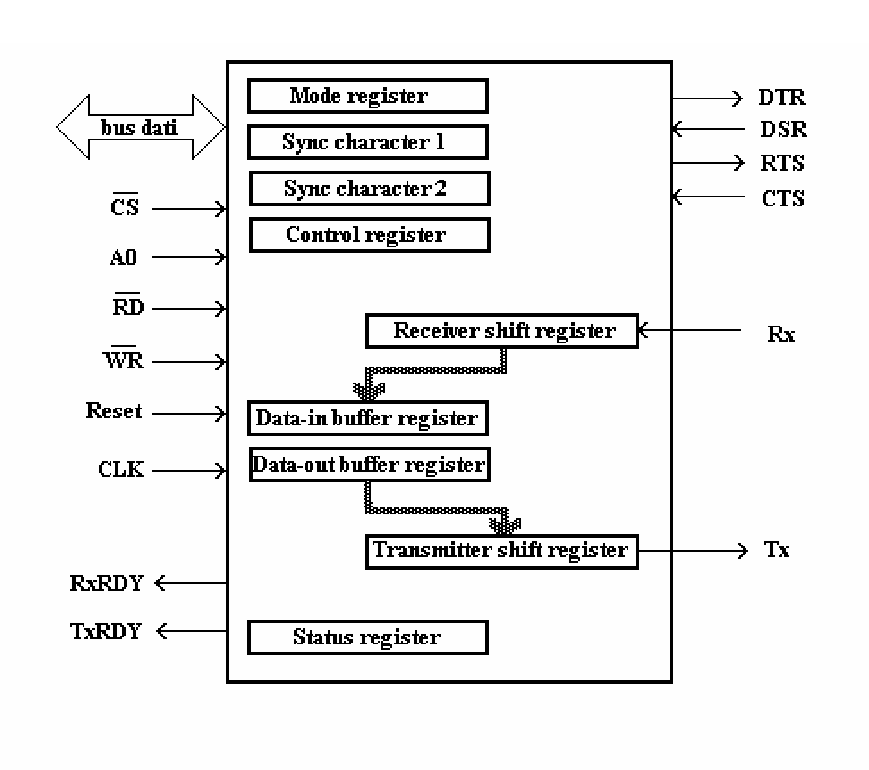
\includegraphics[width=.5\textwidth]{img/prog-8251A.png}
    \caption{Modello di programmazione dell'8251A simulato}\label{img:prog-8251A}
\end{figure}

Da tale figura dobbiamo discriminare due lati, quello sinistro, che è quello che viene connesso direttamente ai bus (e quindi al processore), mentre quello a destra è di interfacciamento verso l'altro dispositivo USART.
Notiamo che i pin sono identici a quelli spiegati nell'architettura generale dell'8251 [\ref{par:intel-8251A}].
Una volta visto il modello di programmazione, vado ad inserire il componente nella mia architettura simulata, quindi lo vado ad inserire all'interno del file di configurazione (.cfg). In generale, come anche per prove precedenti, tali file vengono passati da terze parti, nel caso si volessero configurare \textit{from scratch} si rimanda al capitolo \ref{par:cfg}.
I registri con cui ci si va ad interfacciare con il motorola 68K sono:
\begin{itemize}
    \item \textbf{Mode}: Regsitro di modo con cui posso configurare il funzionamento della USART, quindi selezionare se la comunicazione sia sincrona o asincrona ed il formato dell'informazione da trasmettere (eventuali bit di parità ecc.);
    \item \textbf{CTRL}: Registro di controllo, che permette di poter pilotare i segnali di utilizzo della USART, utile per quando si devono implementare sistemi che utilizzano handshacking ecc.;
    \item \textbf{SYNCH-1}: Registro di Sincronizzazione, utilizzato nella comunicazione sincrona per prevedere l'arrivo del primo simbolo di sincronizzazione;
    \item \textbf{SYNCH-2}: Registro di sincronizzazione, utilizzato nella comunicazione sincrona per prevedere l'arrivo dell'eventuale secondo simbolo di informazione (dipende dalla modalità che si è settata);
\end{itemize}

Per accedere a tali registri di gestione del dispositivo si fa riferimento all'indirizzo dispari messo a disposizione all'interno del file di configurazione. In generale, tali registri, non hanno ognuno il suo puntatore, ma condividono lo stesso indirizzo, che, in base alla tipologia di funzionamento e di impostazione ne permette l'accesso. Precisamente, ogni volta che si fa un accesso in scrittura all'indirizzo dispari si segue l'ordine che è mostrato all'interno dell'immagine [\ref{img:accesso-registri}].

\begin{figure}
    \centering
    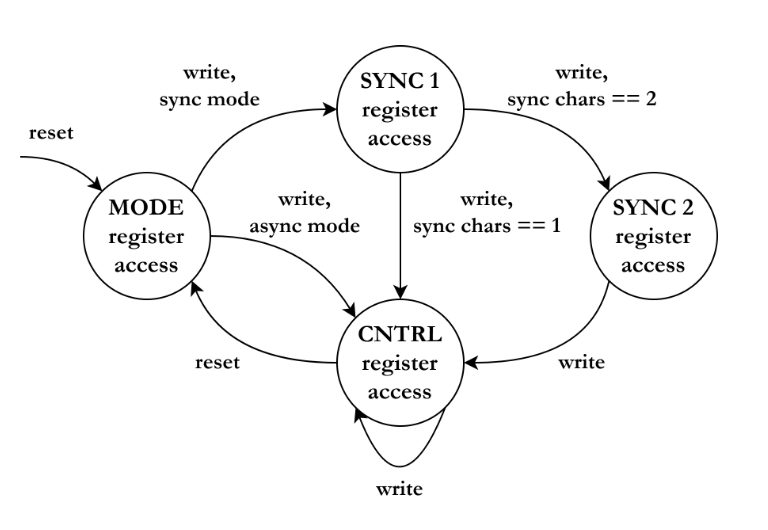
\includegraphics[width=.5\textwidth]{img/registri-8251A.png}
    \caption{Ordine di accesso all'indirizzo dispari}\label{img:accesso-registri}
\end{figure}
Tali però non sono gli unici registri presenti, poichè sono presenti anche i registri di dato (uno per l'ingresso ed uno per l'uscita) ed il registro di stato, per accedere a tali registri si accede, per il registro di stato, in lettura all'indirizzo dispari, mentre per gli indirizzi di dato si accede, in scrittura all'indirizzo pari per il registro d'uscita (DATAOUT), mentre si accede in lettura al registro pari per l'accesso per il registro di ingresso (DATAIN). Di seguito vi sono le tabelle che presentano la struttura dei registri di gestione (Modo, controllo e stato) [\ref{tab:MODE-8251},\ref{tab:CNTRL-8251},\ref{tab:STAT-8251}] e le modalità di accesso ai differenti registri [\ref{tab:accessi}]
\begin{table}[h]
    \centering
    \begin{tabular}{|c|c|l|}
    \hline
    \textbf{Indirizzo} & \textbf{Tipo di accesso} & \textbf{Registro selezionato} \\
    \hline
    Pari   & Lettura (R) & DATIN \\
    Pari   & Scrittura (W) & DATOUT \\
    Dispari & Lettura (R) & STATUS \\
    Dispari & Scrittura (W) & MODE, CNTRL, SYNC1, SYNC2 \\
    \hline
    \end{tabular}
    \caption{Accessi ai registri in base all'indirizzo e tipo}\label{tab:accessi}
\end{table}
    
\begin{table}[h]
    \centering
    \begin{tabular}{|c|p{11cm}|}
    \hline
    \textbf{Bit} & \textbf{Significato} \\
    \hline
    0 & Determina il tipo di trasmissione: 0 per sincrona, 1 per asincrona. \\
    1 & Non utilizzato. \\
    2-3 & Numero di bit d'informazione per carattere: 00 = 5 bit, 01 = 6 bit, 10 = 7 bit, 11 = 8 bit. \\
    4 & Abilita la presenza del bit di parità (1 = presente). \\
    5 & Tipo di parità: pari se 1, dispari se 0. \\
    6 & In modalità asincrona: 0 = 1 bit di stop, 1 = 2 bit di stop. \\
    7 & In modalità sincrona: 0 = 1 carattere di sincronismo, 1 = 2 caratteri. \\
    \hline
    \end{tabular}
    \caption{Significato dei bit del registro MODE}\label{tab:MODE-8251}
\end{table}
    
\begin{table}[h]
    \centering
    \begin{tabular}{|c|p{11cm}|}
    \hline
    \textbf{Bit} & \textbf{Significato} \\
    \hline
    0 & Abilita il trasmettitore. \\
    1 & Attiva il segnale di handshaking DTR. \\
    2 & Abilita il ricevitore. \\
    3 & Non utilizzato. \\
    4 & Cancella i 3 bit d'errore nel registro STATUS. \\
    5 & Attiva il segnale di handshaking RTS. \\
    6 & Resetta l'interfaccia seriale. \\
    7 & Pone il ricevitore nello stato ``hunt'' per cercare i caratteri di sincronismo. \\
    \hline
    \end{tabular}
    \caption{Significato dei bit del registro CNTRL}\label{tab:CNTRL-8251}
\end{table}

\begin{table}[h]
    \centering
    \begin{tabular}{|c|p{11cm}|}
    \hline
    \textbf{Bit} & \textbf{Informazione indicata se posto ad 1} \\
    \hline
    0 & È stato copiato il carattere da DATOUT in TSHIFT (inizio trasmissione). Si azzera alla scrittura successiva. \\
    1 & Un carattere è stato ricevuto in RSHIFT e copiato in DATIN. Si azzera alla lettura. \\
    2 & In trasmissione sincrona, il trasmettitore è privo di dati. \\
    3 & È stato rilevato un errore di parità. \\
    4 & È stato rilevato un errore di overrun. \\
    5 & È stato rilevato un errore di framing. \\
    6 & È stato rilevato il/i caratteri di sincronismo previsti. \\
    7 & È stato attivato il segnale di handshaking DSR. \\
    \hline
    \end{tabular}
    \caption{Significato dei bit del registro STATUS}\label{tab:STAT-8251}
\end{table}
    
  